%%%%%%%%%%%%%%%%%%%%%%%%%%%%%%%%%%%%%%%%%
% University Assignment Title Page 
% LaTeX Template
% Version 1.0 (27/12/12)
%
% This template has been downloaded from:
% http://www.LaTeXTemplates.com
%
% Original author:
% WikiBooks (http://en.wikibooks.org/wiki/LaTeX/Title_Creation)
%
% License:
% CC BY-NC-SA 3.0 (http://creativecommons.org/licenses/by-nc-sa/3.0/)
% 
% Instructions for using this template:
% This title page is capable of being compiled as is. This is not useful for 
% including it in another document. To do this, you have two options: 
%
% 1) Copy/paste everything between \begin{document} and \end{document} 
% starting at \begin{titlepage} and paste this into another LaTeX file where you 
% want your title page.
% OR
% 2) Remove everything outside the \begin{titlepage} and \end{titlepage} and 
% move this file to the same directory as the LaTeX file you wish to add it to. 
% Then add \input{./title_page_1.tex} to your LaTeX file where you want your
% title page.
%
%%%%%%%%%%%%%%%%%%%%%%%%%%%%%%%%%%%%%%%%%
%\title{Title page with logo}
%----------------------------------------------------------------------------------------
%	PACKAGES AND OTHER DOCUMENT CONFIGURATIONS
%----------------------------------------------------------------------------------------

\documentclass[12pt]{article}
\usepackage[english]{babel}
\usepackage[utf8x]{inputenc}
\usepackage{amsmath}
\usepackage{amsfonts}
\usepackage{mathtools}
\DeclarePairedDelimiter{\ceil}{\lceil}{\rceil}
\usepackage{dsfont}
\usepackage{float}
\usepackage{pdfpages}
\newcommand{\ti}{$ \tau_{i} $}
\usepackage{algorithm}
\usepackage[noend]{algpseudocode}

\usepackage{graphicx}
\usepackage{hyperref}
\hypersetup{
    colorlinks,
    citecolor=black,
    filecolor=black,
    linkcolor=black,
    urlcolor=black
}
\usepackage[colorinlistoftodos]{todonotes}
\usepackage[
top    = 3cm,
bottom = 4cm,
left   = 3cm,
right  = 3cm]{geometry}
\begin{document}

\begin{titlepage}

\newcommand{\HRule}{\rule{\linewidth}{0.5mm}} % Defines a new command for the horizontal lines, change thickness here

\center % Center everything on the page
 
%----------------------------------------------------------------------------------------
%	HEADING SECTIONS
%----------------------------------------------------------------------------------------

\textsc{\Large Oral exam INFO-F-404}\\[0.5cm] % Major heading such as course name
\textsc{\large Real-Time Operating Systems}\\[0.5cm] % Minor heading such as course title

%----------------------------------------------------------------------------------------
%	TITLE SECTION
%----------------------------------------------------------------------------------------

\HRule \\[0.4cm]
{ \huge \bfseries Exam's questions}\\[0.4cm] % Title of your document
\HRule \\[1.5cm]
 
%----------------------------------------------------------------------------------------
%	AUTHOR SECTION
%----------------------------------------------------------------------------------------
% If you don't want a supervisor, uncomment the two lines below and remove the section above
Mourad \textsc{Akandouch}\\[0cm] % Your name
Daoud  \textsc{Yemni}\\[0cm] % Your name
       \textsc{         }\\[2cm] % Your name
%----------------------------------------------------------------------------------------
%	DATE SECTION
%----------------------------------------------------------------------------------------

{\large \today}\\[3cm] % Date, change the \today to a set date if you want to be precise

%----------------------------------------------------------------------------------------
%	LOGO SECTION
%----------------------------------------------------------------------------------------

\includegraphics{logo.jpg}\\[1cm] % Include a department/university logo - this will require the graphicx package
 
%----------------------------------------------------------------------------------------

\vfill % Fill the rest of the page with whitespace

\end{titlepage}

\tableofcontents
\newpage
\section{Introduction}
    \paragraph{}
    "The exam is individual, oral without notes/books/papers. You will
    receive two questions related to two different chapters. You have
    half an hour to prepare your answers (blackboard). Then I will
    study your answers and start discussions including sub-questions
    on the same subject, details, sometimes examples, etc.
    My goal is to catch the level of your understanding from superfi-
    cial (fail) to very deep (success). It is not crucial to use the very
    same examples/arguments/notations than mine, but I will check the
    correctness and the understanding of the topics." - Joël Gossens
%----------------------------------------------------------------------------------------
%	CHAPTER 1 - Uniprocessor scheduling
%----------------------------------------------------------------------------------------
\section{Uniprocessor scheduling}
\subsection{Provide two necessary conditions for the feasibility of periodic task systems.}
\begin{itemize}

  \item La première condition nécessaire est que le système $\tau$ doit avoir un facteur
        d'utilisation $U$ inférieur à 1. 
   		En effet, si celui-ci venait à dépasser ce seuil, fatalement, aucun monoprocesseur 
        pourrait scheduler ce système. $U$ étant défini comme la somme de chaque $U_{i}$ de 
        $\tau$. Et $U$ étant également défini comme  : 
        \begin{equation}
          U = \sum\limits_{i=1}^n \frac{C_{i}}{T_{i}}
        \end{equation}        
   \item Les computations time (temps d'exécution) $C_{i}$ des tâches du système doivent 
   		 toutes être inférieures ou égales à leur deadline $D$, sinon elles la manqueront
         toujours. 
         
\end{itemize}

\subsection{Give a periodic implicit deadline systems not schedulable (using RM) with \texorpdfstring{$U < 1$}{Lg}.} % texorpdf parce que Latex n'aime pas les math avec hyperref donc on contourne le probleme avec cette commande
\paragraph{}
Il existe une valeur qui, si le $U$ de notre système y est inférieur ou égal, RM pourra toujours arriver à le scheduler. Cette valeur vaut : 
\begin{equation}
n(\sqrt[n\,]{2} - 1)
\end{equation} où $n$ est le nombre de tâches du système.
Ainsi, on peut d'ores et déjà chercher un système qui viole cette condition suffisante (mais pas nécessaire).
Donc, le système suivant par exemple ($O_{i} = 0$)
  \begin{center}
    \begin{tabular}{| l | c | c |}
      \hline
                   & C  & D = T  \\
      \hline
       $\tau_{1}$  & 4 & 10      \\
      \hline
       $\tau_{2}$  & 3 & 15      \\
      \hline       
      $\tau_{2}$   & 7 & 20      \\
      \hline
  \end{tabular}
  \end{center}




\subsection{Prove the fact that the critical instant occurs when \texorpdfstring{$\tau_{k}$}{Lg} is released at the same time as a job of every higher priority task.}

\paragraph{Définition} Un instant critique d'une tâche \ti est un instant tel que le job de \ti lancé à l'instant où le temps de réponse est maximal et ce, par rapport à tous les jobs de \ti. Informellement, l'instant critique représente le pire scénario parmi tous les jobs de \ti.

\paragraph{}\textit{(Le temps de réponse est le completion time moins le release time)}

\paragraph{Lemme} Un instant critique de n'importe quelle tâche \ti se produit lorsqu'un des jobs $J_{i, k}$ de \ti est release au même moment qu'un job de toute tâche de plus grande priorité.

\paragraph{Croquis de preuve} Soit :
\begin{itemize}
\item $t'$ le release time de $J_{i, k}$
\item $t_{-1}$ le dernier idle instant de toutes les tâches à l'instant (ou avant) $t'$.
\item $t_{R}$ dénote l'instant où $J_{i, k}$ se termine.
\end{itemize}

\begin{figure}[H]
\centering
\includegraphics[width=0.7\textwidth]{img_2_3__0}
\end{figure}

\newpage
\subsection{Prove the optimality of RM in the FTP class.}
\paragraph{Théorème} RM est FTP-optimal pour l'assignement de priorité concernant les tâches synchrones à deadline implicite.

\paragraph{Preuve}
Soit $\tau = \{\tau_{1}...\tau_{n}\}$ un système de tâches périodiques (ou sporadiques) synchrones à deadline implicite. Nous devons prouver que si un assignement de priorité FTP-faisable existe, alors un assignement de priorité RM l'est également.

\paragraph{}
Supposons que l'assignement de priorité FTP-faisable correspond à $\tau_{1} \succ ... \succ \tau_{n}$. Soit \ti et $\tau_{i+1}$ deux priorités adjacentes avec $\tau_{i} \succ \tau_{i+1}$. Échangeons les priorités de \ti et $\tau_{i+1}$...

\paragraph{}\textit{"Ce que RM va faire, c’est swapper deux tâches à chaque fois qu’une tâche a une période plus longue que la suivante. 
En montrant que le swap préserve la faisabilité de l’ensemble des tâches, on a prouvé ce qu’on veut. Pour prouver ça, on dit que les tâches avant \ti ne vont pas changer (elles ont une haute priorité, elles se fichent de ce qu’il y a en-dessous). 
Les tâches après $\tau_{i+1}$ ne changent pas non-plus, car elles ne sont ordonnées que dans les espaces libres laissés par les tâches au-dessus. 
Comme tout ordonnanceur (donc quelque soient les priorités) laisse le CPU libre aux mêmes instants, modifier les tâches au-dessus d’une autre ne change pas l’ordonnancement de cette tâche.}

\paragraph{}\textit{La tâche $\tau_{i+1}$ qui gagne en priorité va bien sûr rester ordonnaçable.
Prouver que la tâche qui diminue de priorité reste ordonnaçable est plus difficile. La tâche qui gagne
en priorité va se terminer plus tôt qu’elle ne le faisait avant. En effet, elle a gagné en priorité, donc elle va commencer plus tôt.}

\paragraph{}\textit{L’instant auquel la tâche qui perd en priorité s’était complétée marquait le début de la période idle du CPU pour l’ensemble des tâches $\tau_{1} ... \tau_{n}$. Comme cette période ne va pas changer (comme vu plus haut), on peut dire que la tâche qui va perdre en priorité va donc se terminer quand la tâche qui a gagné en priorité s’était terminée. Comme cette tâche avait une plus longue période, si la tâche qui a gagné en priorité était on-time, alors celle qui perd en priorité l’est
aussi. Ceci achève la démonstration."} - Denis Steckelmacher, dans son résumé d'OS II sur dochub.be

\subsection{For FTP class, synchronous systems, arbitrary deadline: show the non-optimality of RM \& DM schedulers. Exhibit the important phenomenon which exists for arbitrary schedule impossible for implicit or constrained deadline.}
\paragraph{Soit le système suivant où DM et RM assignent les mêmes priorités ($\tau_{1} \succ \tau_{2}$)}
  \begin{center}
    \begin{tabular}{| l | c | c | c |}
      \hline
                   & C  & D    & T  \\
      \hline
       $\tau_{1}$  & 52 & 110 & 100 \\
      \hline
       $\tau_{2}$  & 52 & 154 & 140 \\
      \hline
  \end{tabular}
  \end{center}
\paragraph{}
Avec cet FTP-assignement de priorité, le premier job de la deuxième tâche rate sa deadline à l'instant 154.
\paragraph{}
Cependant, il est à noter que système reste FTP-faisable si on considère $\tau_{2} \succ \tau_{1}$.

\paragraph{} Sachant qu'on considère des tâches à deadline arbitraires, plusieurs jobs de la même tâche peuvent être actif simultanément. Dans ce cas, l'ordonnanceur ne considère que le job le plus vieux, c'est-à-dire qu'une FIFO est utilisée au niveau de la tâche. (Dans l'exemple ci-dessus, c'est le cas dans l'intervalle $[100, 102]$.)

\paragraph{} Un autre phénomène qui apparaît, c'est le temps de réponse de la première requête qui n'est pas nécessairement le maximum (cf. l'ordonnancement du système où le temps de réponse du premier job est 104 tandis que le second est plus grand).


\subsection{For FTP class, synchronous systems, arbitrary deadline: provide and prove correct a feasibility interval.}
\paragraph{Rappel 1} $\lambda_{i}$ est le premier idle point (après 0) dans l'ordonnancement synchrone du sous-ensemble de tâche $\{\tau_{1}...\tau_{i}\}$, et $[0, \lambda_{i}[$ est la plus grande level-i busy période.
\paragraph{Rappel 2} Une busy période élémentaire est un intervalle de temps $[a, b[$ tel que $a$ et $b$ sont des idle points et l'intervalle $]a,b [$ ne contient aucun idle points.

\paragraph{Rappel 3} Une level-i busy période est une busy période élémentaire en considérant l'ordonnancement des tâches $\{\tau_{1}...\tau_{i}\}$ où \ti exécute au moins un job.

\paragraph{Théorème} Pour un système de tâche synchrone à deadline arbitraire, un intervalle de faisabilité correct est donné par : $[0, \lambda_{n}[$

\paragraph{Preuve} Il s'agit d'une conséquence direct de $\lambda_{1} < \lambda_{2} < ... < \lambda_{n}$
\paragraph{}
$\lambda_{n}$ est la plus petite solution à l'équation :
\begin{equation}
\lambda_{n} = \sum_{i=1}^{n} plafond \left(\frac{\lambda_{n}}{T_{i}} \right) \times C_{i}
\end{equation}
\paragraph{} Et peut être calculé itérativement via :
\begin{equation}
w_{0} = \sum_{i=1}^{n}C_{i} \quad \text{ et } \quad
w_{k} = \sum_{i=1}^{n} plafond\left(\frac{w_{k-1}}{T_{i}} \right) \times C_{i}
\end{equation}


\subsection{For FTP class, synchronous systems and constrained deadline: provide and prove correct a necessary and sufficient schedulability test.}
\paragraph{Théorème} Un système sera FTP-ordonnancable ssi $r_{i}^{1} \leq D_{i} \quad \forall i$

\paragraph{Preuve} Audsley et Tindell ont prouvé que cette quantité est la plus petite solution positive à l'équation :
\begin{equation}
r_{i}^{1} = C_{i} + \sum_{j=1}^{i-1} plafond \left(\frac{r_{i}^{1}}{T_{j}} \right) \times C_{j}
\end{equation}
\paragraph{}
En effet, l'intervalle $[0, r_{i}^{1}[$ inclut $plafond \left(\frac{r_{i}^{1}}{T_{j}} \right)$ requêtes de priorité supérieure en provenance de la tâche $\tau_{j}$.
\paragraph{} À noter également que $r_{i}^{1}$ apparaît des deux côtés de l'égalité. Nous pouvons résoudre cela en passant par une résolution par itération :
\begin{equation}
w_{0} = C_{i} \quad \text{ et } \quad
w_{k+1} =  C_{i} + \sum_{j=1}^{i-1} plafond \left(\frac{w_{k}}{T_{j}} \right) \times C_{j}
\end{equation}
L'itération continue jusqu'à ce que $w_{k+1} = w_{k}$ ou $w_{k} > D_{i}$.

\subsection{For FTP class, asynchronous systems, constrained deadline: prove the property about the schedule periodicity.}
\paragraph{Théorème} Pour des systèmes de tâches asynchrones à deadline contraintes, $[O_{max}, O_{max} + 2P[$ est un intervalle de faisabilité.

\paragraph{} (Tout d'abord, Notez que les intervalles de faisabilité sont périodiques)

\paragraph{Théorème} Les ordonnancements faisables de tâches périodiques sont périodiques (= ces ordonnancements sont périodiques)

\paragraph{Preuve} Pour n'importe quel instant $t > O_{max}$, notons la configuration d'un ordonnancement faisable par le tuple suivant : $(\epsilon_{i}, \delta_{i})$ où $i = 1...n$, $\epsilon_{i}$ est le temps CPU cumulé utilisé par le job courant de \ti et $\delta_{i}$ est le temps écoulé depuis sa dernière requête. Puisque la configuration de l'ordonnancement $S$ au temps $t+1$ est déterminé de manière univoque par la configuration au temps $t \geq 0$ et le fait que tout $i$ ;
\begin{enumerate}
\item $\epsilon_{i}(t) \in [0, C_{i}]$ (le temps utilisé par un job d'une tâche est compris entre 0 et son $C$);
\item $\delta_{i}(t) \in [0, T_{i}]$ (le temps écoulé depuis la dernière requête de la tâche est compris entre 0 et sa période),
\end{enumerate}alors il existe une infinité de configurations possibles et nous pouvons trouver deux instants $t_{1}$, $t_{2}$ (avec $t_{1} < t_{2}$) possédant la même configuration. Ainsi, à partir de $t_{1}$, l'ordonnancement va se répêter périodiquement (avec une période divisant $t_{2} - t_{1}$).

\paragraph{}
\textit{La longueur du cycle est de $P$, et le $2P$ vient du fait qu’on ne sait pas exactement quand le cycle commence, donc il faut s’assurer de simuler le système pendant au moins le temps nécessaire.
Note : À tout instant, le temps processeur déjà alloué à un job est compris entre 0 et le temps d’exécution du job. 
De même, la différence entre l’instant de libération du job et l’instant courant est comprise entre 0 et la deadline. Comme on travaille dans les naturels, il n’y a qu’un ensemble fini de ces valeurs, donc un ensemble fini de leurs combinaisons pour toutes les tâches, ce qui prouve que tout
système d’ordonnancement en temps discret est périodique.} - Denis Steckelmacher, dans son résumé disponible sur dochub.be

\subsection{For FTP class, asynchronous systems, constrained deadline: prove correct the feasibility interval [0, Sn + P]. Explain the meaning of the Si instants.}
\paragraph{Théorème} Pour n'importe quel système de tâches asynchrones à deadlines contraintes ordonné (décroissant) par priorité, soit $S_{i}$ défini récursivement par $S_{1} = O_{1}$, $S_{i} = O_{i} + plafond \left( \frac{(S_{i-1} - O_{i})^{+}}{T_{i}}  \right) \times T_{i}$ et $i=1...n$ ; alors si l'ordonnancement est faisable jusqu'à $S_{n} + P$, avec $x^{+} = max(x, 0)$, alors c'est faisable et périodique à partir de $S_{n}$ avec une période valant $P$ ( = l'hyper-period). 

\paragraph{Preuve} La preuve se fait par induction sur $n$.
\begin{enumerate}
\item La priopriété est OK pour le cas $n=1$ : L'ordonnancement pour $\tau_{1}$ est périodique de période $T_{1}$ à partir de la première release de $\tau_{1} (S_{1} = O_{1})$.
\item Supposons que la propriété soit vraie pour le cas $i-1$ et que l'ordonnancement des $i$ premières tâches est faisable jusqu'à $S_{i} + P_{i}$, avec $Pi = PPCM(T_{j} | j = 1...i)$.
\paragraph{}
$S_{i}$ correspond à la première release de $\tau_{i}$ après (ou en même temps que) $S_{i-1}$ ; Ainsi, $S_{i} \geq S_{i-1}$, $\quad P_{i} \geq P_{i-1}$, $\quad S_{i} + P_{i} \geq S_{i-1} + P_{i-1}$ et par hypothèse d'induction, l'ordonnancement du sous-ensemble de tâches $\{\tau_{1}...\tau_{i-1}\}$ est faisable et périodique de $S_{i-1}$ avec une période $P_{i-1}$. Sachant que les tâches sont ordonnées par priorité, la périodicité des premiers reste inchangée par les requêtes de la tache \ti, et l'ordonnancement se répête au temps $S_{i} + PPCM(P_{i-1}, T_{i})$. Du coup, pour le système $\{\tau_{1}...\tau_{i}\}$, l'ordonnancement est faisable et se répête à partir de $S_{i}$ et avec une période $P_{i}$.
\end{enumerate}
\paragraph{}
Il s'en suit que $[0, S_{n} + P[$ est un intervalle de faisabilité.

\newpage
\subsection{For FTP class, asynchronous systems, constrained deadline: compute the Si values for the following system (O, C, T) : (6, 1, 10), (5, 1, 5), (0, 1, 3) and then check the schedulability.}
\paragraph{ATTENTION : PETITE ERREUR, l'intervalle de faisabilité est $[0, 12 + 30[ = [0, 42[$ !!!}
\begin{figure}[H]
\centering
\caption{Solution de la question 2.10}
\includegraphics[scale=0.33]{img_2_10__0}
\end{figure}



\subsection{For FTP class, asynchronous systems, constrained deadline: using a counter-example, show the nonoptimality of RM and DM priority assignments.}

Considérons le système 
  \begin{center}
    \begin{tabular}{| l | c | c | c |}
      \hline
                   & C  & D = T  & O  \\
      \hline
       $\tau_{1}$  & 1  & 12     & 10 \\
      \hline
       $\tau_{2}$  & 6  & 12     & 0  \\
      \hline
       $\tau_{3}$  & 3  & 8      & 6  \\
      \hline
  \end{tabular}
  \end{center}
\paragraph{} 
Avec l'assignement de priorité $\tau_{3} \succ \tau_{1} \succ \tau_{2}$, l'ordonnancement échoue avec DM et RM malgré qu'il soit FTP-ordonnancable selon l'assignement de priorité $\tau_{3} \succ \tau_{2} \succ \tau_{1}$.
\subsection{For FTP class, asynchronous systems, constrained deadline: provide and prove correct the main property foundation of the optimal Audsley’s priority assignment.}

\paragraph{Propriété} Supposons que $\tau_{i}$ ait la priorité viable la plus basse. Alors, il existe un FTP-assignement faisable pour $\tau$ ssi il existe un assignement de FTP-priorité pour $\tau \setminus  \{ \tau_{i} \} $.

\paragraph{Preuve} Tout d'abord, notons la tâche/la priorité de l'assignement avec $p(\tau_{a}) = b$ signifiant que la priorité de $\tau_{a}$ vaut $b$. Supposons que l'assignement de priorité suivant soit faisable pour $\tau$ :

\begin{equation*}
p(\tau_{1}) = 1, \quad p(\tau_{2}) = 2,... \quad p(\tau_{i}) = i, \quad p(\tau_{i+1}) = i + 1,... \quad p(\tau_{n}) = n
\end{equation*}
\paragraph{}
Alors, un second assignement de priorité est aussi bien faisable :
\begin{equation*}
p'(\tau_{1}) = 1,... \quad p'(\tau_{i+1}) = i, \quad p(\tau_{i+2}) = i + 1,... \quad p(\tau_{n}) = n-1, \quad p(\tau_{i}) = n
\end{equation*}
\paragraph{}
On a simplement mis la $i^{eme}$ tâche à la fin pour qu'elle ait la priorité la plus basse. Ce qui a pour conséquence que les tâche 1 à $i-1$ restent tels quels et donc reste schédulable tandis que les tâches qui avaint la position $i+1$ à $n$ ont gagné une petite priorité car elles se sont décalées d'un cran vers la gauche et restent schédulable.

\subsection{For FTP class, asynchronous systems, constrained deadline: apply the Audsley’s algorithm on the following system (O1 = 2, C1 = 2, D1 = 3,T1 = 4; O2 = 0, C2 = 3, D2 = 4,T2 = 8).}


\subsection{Prove the strong optimality of EDF.}
\textit{" On dit que EDF a une \textbf{strong optimality} car EDF ne regarde que les jobs et ordonnance donc
tout ensemble de travaux. Cela marche donc pour des systèmes synchrones, asynchrone, avec des deadlines arbitraires, ...
\paragraph{}
Il est donc beaucoup plus puissant que FTP et RM/DM. "} 

\paragraph{}
$\#Resume$

\subsection{For EDF, implicit deadline systems: prove the fact that \texorpdfstring{$U \leq 1$}{Lg} is necessary and sufficient.}
\paragraph{Théorème} 
$U(\tau) \leq 1$ est une condition nécessaire et suffisante pour la faisabilité d'un système de tâches périodiques à écheance sur requête.

\paragraph{Preuve} Soit $\tau$ un système de $n$ tâches périodiques à échéances sur requête $\tau_{1}...\tau_{n}$.
Considérons un ordonnanceur "processeur sharing" $S$ obtenu en partitionnant la timeline en unités infinitésimaux et en ordonnancant la tâche $\tau_{i}$ pour une fraction de $U(\tau_{i})$ dans chaque unité de temps. Sachant que $U(\tau) \leq 1$, un tel ordonnancement peut être construit. Cet ordonnancement contient, pour chaque job de $\tau_{i}$, exactement $U(\tau_{i}) \times \tau_{i} = C_{i}$ unités de temps CPU entre l'arrivée du job et sa deadline.

\subsection{For EDF, synchronous systems, constrained deadline: provide the feasibility interval and the procedure to determine its upper-bound.}
\paragraph{Théorème} Lorsque EDF ordonnance un système périodique synchrone à deadline contrainte, il n'y a aucun temps oisif ( = idle) dans l'ordonnancement avant qu'une deadline ne soit manquée.

\paragraph{} 
Il s'en suit que $[0, L[$ est un intervalle de faisabilité pour le système, où  $L$ correspond au premier instant idle (excepté l'origine) dans l'ordonnancement. Cette quantité $L$ peut être trouvée suivant la procédure suivante : 
\begin{equation}
L = \sum_{i=1}^{n}plafond \left( \frac{L}{T_{i}} \right) \times C_{i}
\end{equation}
\paragraph{}
et peut être calculé par itération via :
\begin{equation}
w_{0} = C_{i} \quad  \text{ et } \quad
w_{k+1} = \sum_{i=1}^{n} plafond \left(\frac{w_{k}}{T_{i}} \right) \times C_{i}
\end{equation}
\paragraph{}
À noter qu'il s'agit exactement de la même valeur que $\lambda_{n}$ introduit pour les ordonnanceur FTP.
\subsection{For EDF, asynchronous systems, arbitrary deadline: provide the feasibility interval and using an example show that both the conditions of the test are required.}

\paragraph{Rappel préliminaire : } Considérant un système de tâche $R$ et un ordonnanceur $S$, nous définissons la configuration à l'instant $t$ comme suit :
\begin{equation}
C_{S} (R,t) = ((\gamma_{1}(t), \alpha_{1}(t), \beta_{1}(t)), \quad ..., \quad (\gamma_{n}(t), \alpha_{n}(t), \beta_{n}(t)))
\end{equation}
\paragraph{} où :
\begin{itemize}
\item $\gamma_{i}(t) = (t - O_{i}) \text{ mod } T_{i} \text{ avec } t \geq O_{i}$  \text{. Sinon, } $\gamma_{i}(t) = t - O_{i}$ ; Il s'agit temps passé depuis la dernière requête de \ti.
\item $\alpha_{i}(t)$ est le nombre de jobs actifs de \ti.
\item $\beta_{i}(t)$ est le temps CPU cumulé utilisé par le job actif le plus vieux de \ti. Si $\alpha_{i}(t) = 0$, alors nous posons $\beta_{i}(t) = 0$ aussi.
\end{itemize}

\paragraph{Théorème} Soit $S$ un ordonnanceur EDF pour $R$, un système périodique asynchrone à deadline arbitraire. $R$ est faisable ssi : 
\begin{enumerate}
\item Aucune deadline n'est manqué dans l'intervalle $[0, O_{max} + 2P[$
\item $C_{s}(R, O_{max} + P) = C_{s}(R, O_{max} + 2P)$ 
\end{enumerate}


\paragraph{Exemple} À noter que les deux conditions ci-dessus sont nécessaires, comme montré par le système suivant :
  \begin{center}
    \begin{tabular}{| l | c | c | c | c |}
      \hline
                    & O  &  C  & D  & T  \\
      \hline
       $\tau_{1}$   & 0  &  2  & 4  & 4  \\
      \hline
       $\tau_{2}$   & 2  &  3  & 7  & 4  \\
      \hline
  \end{tabular}
  \end{center}

\paragraph{}
Nous avons que $P = 4$ et $O_{max} = 2$ ; et comme nous pouvons le constater, aucune deadline n'est manquée dans l'intervalle $[0, 10[$ mais $C_{S}(R, 6) \neq C_{S}(R, 10)$, puisque $\beta_{2}(6) = 2$ et $\beta_{2}(10) = 1$. En fait, $\tau_{2}$ manque sa deadline au temps $t = 21$.

\begin{figure}[H]
\centering
\includegraphics[width=\textwidth]{img_2_17__0}
\end{figure}
\paragraph{} Formellement, $[0, O_{max} + 2P[$ n'est pas un intervalle de faisabilité ! \footnote{Définition : Un intervalle de faisabilité est un intervalle de temps fini tel que, si aucune deadline n'est manquée en considérant que les jobs relâchés durant cet intervalle, alors nous pouvons conclure qu'aucune deadline ne sera jamais manquée durant tout le temps de vie du système (c-a-d le système de tâche est faisable)} Notez que la condition $U(\tau) \leq 1$ n'est pas satisfaite par notre système ($U = 1.25$).
\paragraph{}
En fait, si $U(\tau) \leq 1$ est satisfait, seule la première condition du théorème doit être satisfaite pour conclure que le système est faisable.


\newpage
\subsection{LLF: define laxity, the priority management and the trashing situation using an example.}
\paragraph{Définition de laxité } Soit un job $J$ caractérisé par le tuple $(a, e, d)$. Soit $\epsilon_{J}(t)$, le temps CPU cumulé utilisé par $J$ depuis son release. La \textbf{laxité} (noté $\ell_{J}(t)$) à l'instant $t$ est définie comme suit : $\ell_{J}(t) =  d − t − (e − \epsilon_{J}(t))$.

\paragraph{LLF : } Least Laxity first est un ordonnanceur à priorité dynamique au niveau du job. LLF est aussi appelé \textit{algorithme temps-mort (ou Temps de folie ?) (=$>$ slack-time algorithm)}

\paragraph{Gestion de priorité} La laxité d'un job représente son degré d'urgence :
\begin{itemize}
\item Si $\ell_{J}(t) > 0$, le job peut être possiblement retardé (avec un maximum de $\ell_{J}(t)$ unité de temps) avant d'être ordonnancé.

\item $\ell_{J}(t) = 0$, il est obligatoire d'ordonnancer le job immédiatement jusqu'à sa deadline pour assurer la faisabilité.

\item $\ell_{J}(t) < 0$ le job va certainement manquer sa deadline.
\item Note : la laxité d'un job actif reste constant.
\end{itemize}

\paragraph{Situation de merde} LLF et EDF sont tout deux optimaux mais ils diffèrent au niveau du nombre de préemptions durant l'ordonnancement. Considérons le système suivant :
  \begin{center}
    \begin{tabular}{| l | c | c | c | c |}
      \hline
                    &  C  & T  & D  \\
      \hline
       $\tau_{1}$   &  4  & 10 & 8  \\
      \hline
       $\tau_{2}$   &  5  & 10 & 8  \\
      \hline
  \end{tabular}
  \end{center}
\paragraph{} EDF ne fera aucune préemption tandis que LLF aura 6 préemptions chaque 10 unités de temps !

\paragraph{Trashing situation} Il s'agit d'une situation où un grand nombre de ressources est utilisé pour faire un petit travail.

\begin{figure}[H]
\centering
\includegraphics[width=\textwidth]{img_2_18__0}
\caption{Ordonnancement du système avec LLF}
\end{figure}

\begin{figure}[H]
\centering
\includegraphics[width=\textwidth]{img_2_18__1}
\caption{Ordonnancement du système avec EDF}
\end{figure}


\newpage
\subsection{Build an LLF schedule for the following system (C,T, D): (1, 3, 3)(4, 5, 6).}
\begin{figure}[H]
\centering
\includegraphics[height=0.7\textheight,width=\textwidth]{img_2_19__0}
\end{figure}


%----------------------------------------------------------------------------------------
%	CHAPTER 2 - Multiprocessor scheduling
%----------------------------------------------------------------------------------------
\newpage
\section{Multiprocessor scheduling}

\subsection{For partitioning scheduling define and compare FF and BF heuristics.}
\paragraph{}
FF (First fit) et BF (Best fit) sont deux heuristiques permettant de donner une solution approximative au problème de Bin Packing considéré comme NP-difficile (NP-hard). Ici, les bins (les boîtes) sont représentés par le nombre de processeurs et les objets à placer sont les tâches d'un système.

\paragraph{}
Concernant First fit, l'algorithme consiste à :
  \begin{enumerate}
    \item Trier les tâches du système par facteur d'utilisation $U$ (croissant ou 
          décroissant).
    \item Itérer sur chaque tâches et placer la tâche courrante sur \textbf{le premier} 
          processeur de libre en partant du début. Par libre, on sous-entend que la 
          charge du processeur choisi + le $U$ de la tâche à placer soit $\leq$ à $1$.
  \end{enumerate}
\paragraph{}
Quant à Best fit, l'algorithme consiste à :
	\begin{enumerate}
      \item Trier les tâches du système par facteur d'utilisation $U$ (croissant ou 
            décroissant).
      \item Itérer sur chaque tâches et placer la tâche courrante sur le processeur qui, 
            si on lui ajoute la tâche courante, aura le $U$ le plus élevé parmi tous les 
            processeurs (eux aussi avec le $U$ de la tâche courante ajoutée).
            Formellement, le processeur choisi sera le processeur correspondant au $max(U(\pi_{1}) + U(\tau_{courant}), U(\pi_{2}) + U(\tau_{courant}), ..., U(\pi_{n}) + U(\tau_{courant}))$
	\end{enumerate}
    
\subsection{For global scheduling prove that no online optimal scheduler exists.}

\paragraph{}
\textit{Théorème de Hong et Leug : Pour n'importe quel nombre de processeur supérieur à 1, il n'existe aucun algorithme d'ordonnancement en ligne qui soit optimal\footnote{[Hong and Leung, 1988] Hong, K. and Leung, J. (1988). On-line scheduling of real-time tasks. In Real-Time Systems Symposium.}}

\paragraph{}
Un ordonnanceur en ligne est un type d'ordonnaceur qui décide \textit{à l'exécution du programme} de choisir quelle tâche va être élue. L'ordonnanceur se basera sur les caractéristiques des jobs déjà relâchés et ne connait absolument rien du futur.

\paragraph{Preuve} (Faites le dessin pour vous représenter la preuve) Considérons le cas où il y a deux processeurs. (Notons $m$ pour le nombre de processeurs) La preuve se fait par contradiction. À l'instant 0, trois jobs $j_{1}, j_{2}, j_{3}$  sont relâchés avec comme deadline $d_{1} = 4, d_{2} = 4, d_{3} = 8$ et comme temps d'exécution $e_{1} = 2, e_{2} = 2, e_{3} = 4$.

\paragraph{} 
L'algorithme va ordonnancer les jobs sur deux processeurs en démarrant à l'instant $t = 0$. Nous pouvons distinguer deux types d'ordonnancement en ligne : 
  \begin{itemize}
    \item \textbf{Premier cas  -} $j_{3}$ est exécuté dans l'intervalle $[0,2[$. Dans ce 
          cas, au moins un des deux autres jobs ($j_{2} ou j_{3}$) ne sera pas 
          \textbf{terminé} à l'instant $t = 2$.
          \paragraph{}
    	  Maintenant, supposons que ce soit le cas pour $j_{2}$, donc qu'il n'a pas fini 
          son exécution à l'instant $t = 2$. Supposons qu'il y ait deux nouveaux jobs 
          $j_{4} = (D = 4, e = 2)$ et $j_{5} = (D = 4, e = 2)$ qui sont relâchés à 
          l'instant $t = 2$. 
          \paragraph{}
          Clairement, on remarque que l'ordonnancement en ligne va manquera des 
          deadlines malgré que le système (5 jobs) soit faisable. L'ordonnanceur 
          n'aurait pas dû exécuter $j_{3}$ durant l'intervalle $[0, 2[$. Mais de toute 
          façon, même choisir de ne pas exécuter $j_{3}$ durant le dit intervalle n'est 
          pas un choix optimal (voir cas suivant).
          
    \item \textbf{Deuxième cas -} Supposons que $j_{3}$ n'ait pas du tout progressé dans 
          l'intervalle $[0, 2[$. Dans ce cas, à l'instant $t = 4$, il reste au moins 
          deux unités de temps d'exécution et $j_{1}, j_{2}, j_{3}$ ont pu se finit.
          \paragraph{}
          Mais, supposons qu'il y ait deux autres jobs $j'_{4} = (D = 8, e = 4)$ et 
          $j'_{5} = (D = 8, e = 4)$ qui sont tout deux relâchés à l'instant $t = 4$. On 
          remarque directement que l'ordonnancement va rater. $j_{3}$ aurait dû 
          s'exécuter durant l'intervalle $[0, 2[$.
  \end{itemize}
  
  \paragraph{}
  De même pour un ensemble de tâches sporadiques, le contre-exemple de Hong concerne 
  l'ordonnancement et ne peut pas être étendu pour montrer la non-existence d'un 
  algorithme d'ordonnancement optimal en ligne multiprocesseur pour un système de tâches 
  sporadiques.

  \paragraph{} Dans \textit{Fisher et al., 2010}\footnote{[Fisher et al., 2010] Fisher, 
  N., Goossens, J., and Baruah, S. (2010). Optimal online multiprocessor scheduling of 
  sporadic real-time tasks is impossible. Real-Time Systems: The International Journal 
  of Time-Critical Computing, 45(1–2):26–71.} notre professeur et ses collègues ont 
  montré que le système de tâches sporadiques suivant est faisable mais il recquiert que 
  nous ayons connaissance du futur, de la clairvoyance.
  \begin{center}
    \begin{tabular}{| l | c | c | c |}
      \hline
                   & C  & D  & T \\
      \hline
       $\tau_{1}$  & 2  & 2  & 5 \\
      \hline
       $\tau_{2}$  & 1  & 1  & 5 \\
      \hline
       $\tau_{3}$  & 1  & 2 & 6  \\
      \hline
       $\tau_{4}$  & 2 & 4 & 100 \\
      \hline     
       $\tau_{5}$  & 2 & 6 & 100 \\
      \hline     
       $\tau_{6}$  & 4 & 8 & 100 \\
      \hline
  \end{tabular}
  \end{center}

\subsection{Define the concept of scheduling anomalies, illustrate the phenomenon for global FTP scheduling and the period parameter.}

  \paragraph{}
  Avant de définir le concept d'anomalies d'ordonnacncement \textit{(scheduling 
  anomalies)}, il faut définir ce qu'est un changement intuitivement positif 
  \textit{(Intuitively positive change)}.

  \paragraph{Changement intuitivement positif : } Il s'agit de n'importe quel changement 
  pouvant faire diminuer le facteur d'utilisation $U$ d'une tâche (augmentation de la 
  période, diminution du temps d'exécution, accélération du processeur).

  \paragraph{Anomalie d'ordonnancement : } Une anomalie d'ordonnancement apparaît 
  lorsqu'un \textit{changement intuitivement positif} d'un des paramètres du système (de 
  tâches, de job ou de la platforme d'exécution) peut compromettre l'ordonnancement du 
  système.
  
  \paragraph{} Soit le système suivant : $\tau_{1} = (T_{1} = 4, D_{1} = 2, C_{1} = 
   1)$, 
   $\tau_{2} (T_{2} =5, D_{2} = 3, C_{2} = 3)$, $\tau_{3} = (T_{3} = 20, D_{3} = 8, 
   C_{3} = 7)$ Ce système est faisable en utilisant DM global. Malheureusement, si nous 
   incrémentons la période de $\tau_{1}$ de 4 à 5, ce même ordonnanceur va faire rater 
   la deadline de $\tau_{3}$ à l'instant $t = 8$.
   \begin{figure}[H]
      \centering
      \includegraphics[width=\textwidth]{img_3_2__0}
      \caption{L'ordonnancement originel sans changement}
   \end{figure}
   \begin{figure}[H]
      \centering
      \includegraphics[width=0.7\textwidth]{img_3_2__1}
      \caption{L'ordonnancement originel \textbf{AVEC} changement}
   \end{figure}
   
\subsection{Define the PFair scheduling rule using the notion of lag.}
\paragraph{}
L'ordonnancement PFAIR (Proportionally fair) est un type d'ordonnancement qui permet l'exécution de tâches à un rythme quasiment constant. Pour des tâches périodiques, chaque tâche s'exécute à un rythme d'environ $U(\tau_{i})$ pour de larges intervalles. Ce taux varie un peu pour de petits intervalles.

\paragraph{}
Avant de définir la notion de lag, il est essentiel de comprendre ce que fait un ordonnancement equitable (fair). 
Un tel ordonnanceur va donner un certain quantum (une portion de temps) à chaque tâches. L'ordonnanceur est appelé à chaque fin de quantum afin d'appeler la tâche suivante à exécuter. Formellement, nous pouvons définir une fonction $S : \tau \times \mathbb{Z} \rightarrow \{0, 1\}$. C'est-à-dire qu'elle reçoit deux arguments (une tâche et un entier) et renvoie un élément de l'ensemble $\{0, 1\}$.
\begin{itemize}
\item $S(\tau_{i}, t) = 1$ signifie qu'au temps $t$, la tâche $\tau_{i}$ s'exécute.
\item $S(\tau_{i}, t) = 0$ signifie qu'au temps $t$, la tâche $\tau_{i}$ \textbf{ne} s'exécute \textbf{pas}.
\end{itemize}

\paragraph{}
L'idée derrière un ordonnancement équitable idéal est que chaque tâche se voit octroyée $U(\tau_{i})\times t$ unités de temps dans l'intervalle $[0, t[$, ce qui implique qu'aucune deadline ne sera ratée. À noter qu'un tel ordonnancement n'est pas nécessairement possible en utilisant des temps discrets (c-à-d entier).

\paragraph{}
Ainsi, l'idée derrière PFAIR est d'imiter un maximum les ordonnanceurs équitables idéaux. À chaque instant, la différence entre l'ordonnancement actuel et celui d'un équitable idéal peut être formalisée par la notion de \textbf{lag} (retard, décalage). Le \textbf{lag} d'une tâche $\tau_{i}$ au temps $t$ se note par $lag(\tau_{i}, t)$ est défini comme suit :
\begin{equation}
lag(\tau_{i}, t) = U(\tau_{i}).t - \sum_{\ell = 0}^{t-1} S(\tau_{i}, \ell)
\end{equation}

\paragraph{}
Et donc, il y a une propriété pour qu'un ordonnanceur soit PFAIR : Pour chaque tâche, et pour tout temps $t$, le lag soit compris entre -1 et 1 (bornes exclues). C'est-à-dire que la différence entre un ordonnanceur équitable idéal et le PFAIR soit toujours inférieure à une unité de temps. Formellement, cela peut s'écrire comme suit :
\begin{equation}
-1 < lag(\tau_{i}, t) < 1, \enspace \enspace \enspace \enspace \enspace \forall \tau_{i} \in \tau, t \in \mathbb{Z}
\end{equation}

\paragraph{Peut-être que le professeur nous demandera des questions corollaires, donc à retenir : }
\begin{itemize}
\item Théorème : être PFAIR implique qu'aucune deadline ne soit ratée.
\item Théorème : Si un système de tâche périodique, synchrone et implicit-deadline voit son $U$ inférieur ou égal au nombre de processeur et le $U$ de toute ses tâches $\leq$ à 1, alors PFAIR peut l'ordonnancer.
\item PFAIR est optimal. Ca ne contredit pas le théorème disant qu'aucun ordonnancement optimal en ligne existe car ici, on ne parle que de tâches périodiques
\end{itemize}

\subsection{Provide the basic sufficient condition for EDF schedulability of implicit deadline tasks, present the EDF(k) improvement.}
\paragraph{Théorème} N'importe quel système de tâche implicit-deadline sporadique peut se faire ordonnancé via global EDF sur $m$ processeur si cette condition est respectée : 
\begin{equation}
U(\tau_{i}) \leq m - (m-1).U_{max}
\end{equation}
\paragraph{}
Cette condition est plutôt pessimiste pour les tâches dont leur $U$ tend vers 1. Heureusement, il existe un algorithme $EDF^{(k)}$ capable de résoudre cet inconvénient.

\paragraph{}
Tout d'abord, considérons une simplification qui permettra d'alléger les notations. Considérons que notre système soit trié tel que : $U(\tau_{1}) \geq U(\tau_{2}) \geq ... \geq U(\tau_{n})$. Également, l'écriture $\tau^{(k)}$ est introduite qui correspond à l'ensemble des tâches de $\tau_{i}$ à $\tau_{n}$. Autrement dit, l'ensemble des tâches avec un facteur d'utilisation inférieur à $U_{i}$ (lui-même compris dans l'ensemble).

\paragraph{}
Du théorème précédent, on peut arriver à cette forme en triturant l'équation : 
\begin{equation}
m \geq \ceil[\Bigg]{\frac{U(\tau) - U(\tau_{1})}{1 - U(\tau_{1})}}
\end{equation}

\paragraph{}
Ainsi, nous pouvons adapter le nombre de processeur pour autant que nous respectons la condition précédente.

\paragraph{} Avant d'avancer plus loin, définissons $EDF^{(k)}$ : 
\begin{itemize}
\item Pour tout $i < k$, les jobs des tâches $\tau_{i}$ recoivent une priorité maximale. (Facilement faisable en mettant leur deadline absolue à $-\inf$).
\item Tous les autres jobs gardent leur priorité normales en accord avec $EDF$.
\end{itemize}

\paragraph{}
En d'autres termes,  $EDF^{(k)}$ donne une priorité maximale aux $k-1$ premières tâches et ordonnance le reste normalement. À noter que l'$EDF$ pure correspond à $EDF^{(1)}$.

\paragraph{Théorème - } "Un système de tâche sporadique et implicit-deadline est ordonnancable via $EDF^{(k)}$ sur $m$ processeurs si"\footnote{[Goossens et al., 2003] Goossens, J., Funk, S., and Baruah, S. (2003).
Priority-driven scheduling of periodic task systems on
multiprocessors.
Real-Time Systems: The International Journal of Time-Critical
Computing, 25:187–205.} : 
\begin{equation}
m = (k-1) + \ceil[\Bigg]{\frac{U(\tau^{(k)})}{1 - U(\tau_{k})}}
\end{equation}
\paragraph{}
En d'autres termes, $EDF^{(k)}$ recquiert un processeur $\pi_{1}$ pour les jobs de la tâche $\tau_{1}$, un processeur $\pi_{2}$ pour les jobs de la tâche $\tau_{2}$... un processeur $\pi_{k-1}$ pour les jobs de la tâche $\tau_{k-1}$ et ordonnance tout le reste via $EDF$ en utilisant un nombre additionnel de processeurs. Au final, il y aura entre $k$ et $(k-1) + \ceil[\Big]{\frac{U(\tau^{(k)})}{1 - U(\tau_{k})}}$ processeurs.


\subsection{Build a global DM schedule for the following system upon two processors (C,T): (1, 2)(2, 4)(6, 8).}
\begin{figure}[H]
	\centering
	\includegraphics[angle=90,width=\textwidth]{img_3_6__0}
    \caption{Réponse 3.6 : Ordonnancement global DM avec deux processeurs}
\end{figure}

\subsection{Build an EDF(k) schedule for the following system upon two processors (C,T): (9, 10)(1, 3)(3, 6).}
\begin{figure}[H]
	\centering
	\includegraphics[scale=0.7]{img_3_7__0}
    \caption{Réponse 3.7 : Ordonnancement global $EDF^{k}$ avec deux processeurs}
\end{figure}

\subsection{Build a PFair schedule for the following system upon two processors (C,T): (2, 3)(2, 3)(4, 6).}
lol trop facile
\subsection{Build a global EDF schedule for the following system upon two processors (C,T): (1, 3)(2, 4)(2, 4).}
   \begin{figure}[H]
      \centering
      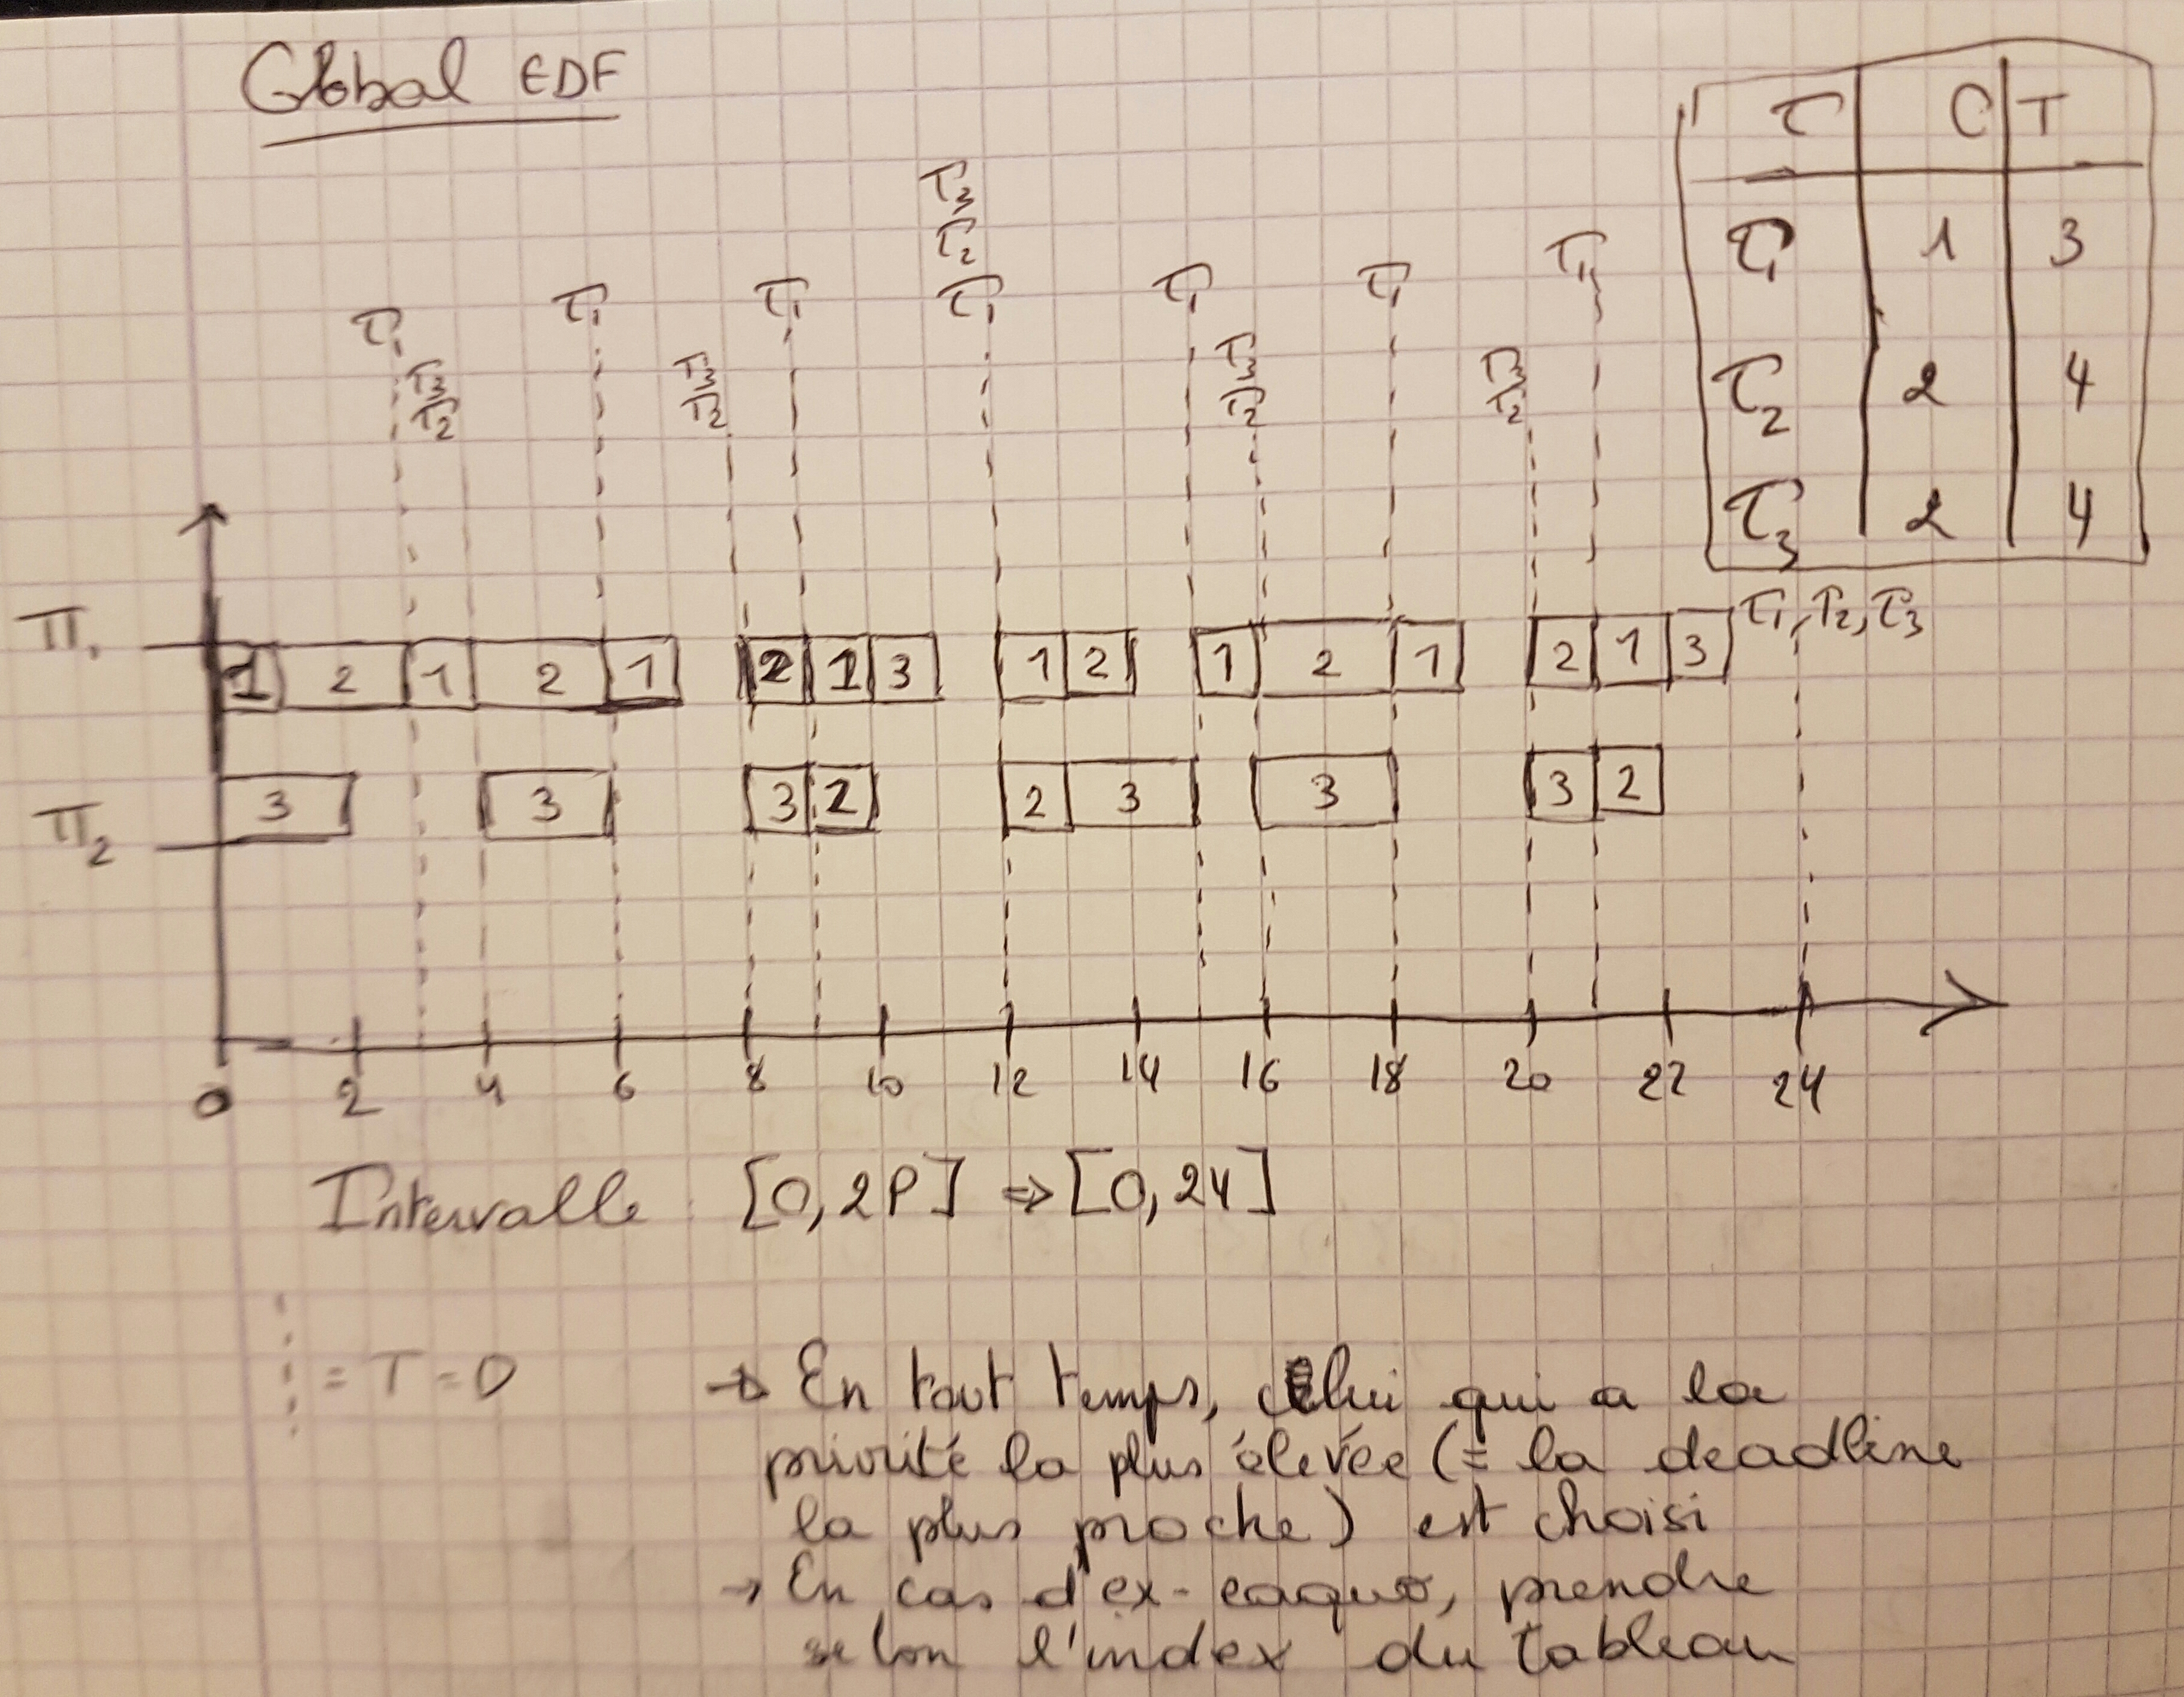
\includegraphics[width=\textwidth]{img_3_9__0}
      \caption{Réponse 3.9 : Ordonnancement global EDF avec deux processeurs}
   \end{figure}
\subsection{Provide a necessary and sufficient condition for the feasibility of implicit deadline systems upon multiprocessors.}

\paragraph{}
Dans le cas d'un assignement partitionné (et non global), un système de tâche est ordonnancable avec EDF en utilisant le partitionnement FFDU (First fir decreasing utilization) si la condition suivante est respectée :
\begin{equation}
U(\tau) \leq \frac{m+1}{2} \quad \textrm{et} \quad U_{max} \leq 1
\end{equation}
\paragraph{}
C'est-à-dire que le facteur d'utilisation total du système soit inférieur ou égal à la moitié du nombre de processeurs + 1. Et que le plus grand facteur d'utilisation parmi toutes les tâches soit également inférieur ou égal à 1.

\subsection{Half-proof of the fact that partitioning and global scheduling are incomparable: system such that a partition exists while all global-FTP schedulers fail.}
Soit le système suivant :
  \begin{center}
    \begin{tabular}{| l | c | c | c |}
      \hline
                   & C  & T  & D  \\
      \hline
       $\tau_{1}$  & 2  & 3  & 2  \\
      \hline
       $\tau_{2}$  & 3  & 4  & 3  \\
      \hline
       $\tau_{3}$  & 4  & 12 & 12 \\
      \hline       
      $\tau_{3}$  &  3  & 12 & 12 \\
      \hline
  \end{tabular}
  \end{center}
  
Lorsqu'on le simule avec un algorithme d'ordonnancement DM (et donc un ordonnanceur FTP) sur deux processeurs, l'assignement partitionné réussit ($\tau_{1, 3}$ pour $\pi_{1}$ et $\tau_{2,4}$ pour $\pi_{2}$) mais en global, $\tau_{3}$ ou $\tau_{4}$ ratera sa première deadline.
%----------------------------------------------------------------------------------------
%	CHAPTER 3 - Concurrency
%----------------------------------------------------------------------------------------
\newpage
\section{Concurrency}
\subsection{Solution to the producer-consumer problem, bounded buffers.}
\paragraph{}
Une solution simple pour résoudre le problème de producteur-consommateur est l'utilisation de deux sémaphores.
La première servira à ne pas introduire de données dans le buffer lorsque celui-ci est déjà plein. Le second permettra au consommateur de ne pas consommer des données si le buffer est vide.
\begin{figure}[H]
	\centering
    \includegraphics[width=0.6\textwidth]{img_4_1__0}
\end{figure}



\subsection{Bakery algorithm}
\paragraph{}
L'algorithme de la boulangerie est une technique permettant la gestion de section critique entre $n$ processus. L'idée étant de simuler le fonctionnement d'une boulangerie : Les processus reçoivent chacun un ticket à l'instar d'un boulanger qui donne des tickets à ses clients pour les servir dans l'ordre. Le numéro des tickets augmente constamment et c'est le process ayant le ticket avec le plus petit numéro qui a droit à entrer en section critique (se faire servir par le boulanger).

\begin{figure}[H]
	\centering
    \includegraphics[width=0.6\textwidth]{img_4_2__0}
\end{figure}
\paragraph{}
Les instructions $p2$ et $p4$ servent à faire de l'instruction $p3$ une section critique car il est irréaliste de penser que la recherche d'un maximum dans un tableau puisse se faire de manière atomique. Cette instruction $p3$ recherche donc le ticket possédant la plus haute valeur et assigne $max+1$ au process courant tout en indiquant aux autre process que le courant est en train d'effectuer cette opération, et donc qu'aucun autre ne doit également le faire pour le moment. (il s'agit là de l'utilité des instructions $p2$ et $p4$.)

\paragraph{}
L'instruction $p5$ à $p7$ font office de pré-protocole pour entrer en section-critique. Une boucle itère sur chaque processus. $p6$ indique que si au moins un process est en train de calculer son numéro de ticket, alors on attend qu'il se termine. $p7$ permet d'attendre que les autres process aient finis leur section-critique \textbf{ou}, que c'est bien notre tour. ($number[i] << number[j]$ est une abbréviation de "\textit{mon ticket possède une valeur inférieur à celui du process $j$ \textbf{ou} nos deux tickets sont ex-aequo mais je possède un identifiant plus petit.}" qui se traduit par : $(number[i] < number[j]) || ((number[i] == number[j]) \&\& (i<j))$)





\subsection{Algorithm of Ricart-Agrawala (distributed critical sections).}
\paragraph{Réponse de Issam}
\includepdf[pages=-,pagecommand={},width=\textwidth]{RTOS_concurence_2_3_3.pdf}






\subsection{Starvation definition. Illustrate the phenomenon using one of the Dekker’s attempts.}
\paragraph{}
La famine est un problème que peut posséder un algorithme. Si celui-ci ne garantit pas une probabilité non-nulle à tous les processus souhaitant accéder à une section critique, alors les processus peuvent être victime de famine.
\paragraph{}
Dans l'algorithme ci-dessous qui est la troisième tentative du cours pour arriver à l'algorithme de Dekker, une famine peut se produire si l'ordonnancement alterne toujours entre une instruction de $p$ puis une instruction de $q$ et ce, éternellement. 
\begin{figure}[H]
	\centering
    \includegraphics[width=0.6\textwidth]{img_4_4__0}
\end{figure}

\subsection{Byzantine Generals algorithm}
L'algorithme des généraux de l'armée Byzantine est une méthode garantissant une solution aux problèmes de consensus. Les problèmes pouvant survenir lors d'un vote et du consensus de la tactique à adopter sont de deux sortes :
\begin{enumerate}
\item Crash failure : Un nœud arrete d’envoyer des messages (facilement détectable au moyen d'un timeout)
\item Byzantine failure : Un nœud envoie des messages erronés ou arbitraires.
\end{enumerate}

\paragraph{Réponse de Issam}
\includepdf[pages=-,pagecommand={},width=\textwidth]{RTOS_concurence_2_3_5.pdf}











%----------------------------------------------------------------------------------------
%	CHAPTER 4 - Parallel programming
%----------------------------------------------------------------------------------------
\section{Parallel programming}
\subsection{Provide the Amdahl’s law and illustrate its consequences.}
\paragraph{}
Initiallement, pour mesurer le facteur d'accélération du temps pris par un algorithme lorsqu'on compare sa version séquentielle et parallélisée, on a recourt à une formule simple : 
\begin{equation}
S(n) = \frac{t_{s}}{t_{p}}
\end{equation}
\paragraph{}
où $t_{s}$ est le temps pris pour exécuter un algorithme donné de manière séquentielle et $t_{p}$ représente le temps pris pour exécuter ce même algorithme mais dans sa version parallélisée. $S(n)$ est le facteur d'accélération. Le facteur d'accélération maximal atteignable est $n$ lorsqu'on utilise $n$ processeurs. 

\paragraph{}
La loi d'Ahmdal nous indique qu'il y aura toujours une limite supérieure quant au nombre de processeurs nécessaire pour paralléliser un algorithme. En effet, un algorithme possèdera toujours une portion de son code qui devra s'exécuter de manière séquentielle (ne serait-ce qu'une simple addition). Posons $f$, le pourcentage représentant la partie séquentielle d'un algorithme. Fatalement, $(1-f)$ représente le pourcentage parallélisable du dit algorithme. Ainsi, le temps total nécessaire à l'exécution de l'algorithme (sachant que le nombre maximum de processeur a été utilisé) est :
\begin{equation*}
t_{p} = \underbrace{f . t_{s}}_\text{Partie séquentielle} +  \underbrace{(1-f) . \frac{t_{s}}{n}}_\text{Partie parallélisable}
\end{equation*}
Ainsi, si on replace dans notre formule originale, cela donne : 
\paragraph{}
La loi d'Ahmdal  : 
\begin{equation}
S(n) = \frac{t_{s}}{f . t_{s} + (1-f) . \frac{t_{s}}{n}}  = \frac{n}{1+(n-1).f}
\end{equation}
\paragraph{}
Une conséquence de cette loi est que lorsque $n$ tend vers l'infini, le facteur d'accélération vaut $\frac{1}{f}$. Ainsi, par exemple, si seulement 5\% d'un algorithme est séquentiel, le facteur maximal d'accélération sera de 20, indépendamment du nombre de processeur que nous fournissons.

\subsection{Bitonic Mergesort: principles, algorithms, complexity.}
Le \textbf{Bitonic Mergesort} est un algorithme qui permet trier indépendamment chaque moitié d'une séquence.
\paragraph{}
\textbf{Définition 1 : Séquence bitonic}
\paragraph{}
Une séquence $(a_1, a_2, ..., a_{2k})$ est dite bitonic ssi il existe un entier $j$ compris entre $1$ et $2k$, tel que : \[a_1 \leq a_2 \leq ... \leq a_j \geq a_{j+1} \geq a_{j+2} \geq a_{2k} \]

\paragraph{}
\textbf{Définition 2 : Compare-and-swap}
\paragraph{}
Le \textbf{Compare-and-swap} est une instruction recevant une paire d'élément distincts et renvoie cette paire dans l'ordre croissant ou décroissant (selon le choix) en 1 unité de temps = O(1).

\paragraph{}
L'algorithme "\textbf{$Merge_{2k}$}" s'effectue en 3 étapes :
\begin{enumerate}
\item On crée 2 séquences $(e_1, e_2,...,e_k)$ et $(d_1, d_2, ..., d_k)$ tel que :
\begin{itemize}
\item $e_{i} = min(a_{i}, a_{k+i})$
\item $d_{i} = max(a_{i}, a_{k+i})$
\end{itemize}
\item On trie les 2 séquences indépendamment en faisant appel à \textit{$Merge_{k}$} (qui est une sous-fonction de \textbf{$Merge_{2k}$} et qui utilise le \textbf{Compare-and-swap}).
\item On concatène les 2 séquences triées et on renvoie la séquence triée complète.
\end{enumerate}

\paragraph{}
\textbf{Exemple :}
\paragraph{}
Nous avons la séquence bitonic suivante : $S = \{3, 5, 8, 9, 7, 4, 2, 1\}$. $2k$ représente la longueur de la séquence $=>$ 8, alors k vaut 4. 
\begin{enumerate}
\item e $<-$ min(3,7) et d $<-$ max(3,7) $=>$ e $\{3\}$ et d $\{7\}$
\item e $<-$ min(5,4) et d $<-$ max(5,4) $=>$ e $\{3,4\}$ et d $\{7,5\}$
\item e $<-$ min(8,2) et d $<-$ max(8,2) $=>$ e $\{3,4,2\}$ et d $\{7,5,8\}$
\item e $<-$ min(9,1) et d $<-$ max(9,1) $=>$ e $\{3,4,2,1\}$ et d $\{7,5,8,9\}$
\end{enumerate}
\paragraph{}
Maintenant nous allons trier les 2 séquences, ce qui nous donne à la fin :
\begin{itemize}
\item e' {1,2,3,4}
\item d' {5,7,8,9}
\end{itemize}
\paragraph{}
Une fois les 2 séquences triées, nous allons concaténer ces 2 séquences et renvoyer le résultat :
S' = $e' \oplus d'$

\paragraph{}
\textbf{Complexité}
\paragraph{}
En considérant que $2k = 2^i$, le temps de $Merge_{2k}$ est donné par la récurrence :
\[d(2) = 1\]
\[d(2^{i}) = 1 + d(2^{i-1}) \]
donc la solution est $d(2^i) = i$. Conséquence, le temps total est :
\[ \sum^{\log{n}}_{i = 1} d(2^i) = \sum^{\log{n}}_{i = 1}i = \frac{(1+\log{n})\log{n}}{2} = O((\log{n})^2)\]
\paragraph{}
La complexité en temps du \textbf{Bitonic Sort} est de $O((\log{n})^2)$.
\paragraph{}
La complexité en temps du \textbf{Compare-and-swap} est de $O(n(\log{n})^2)$.

\subsection{Main principles and properties which allows to parallelize the simulation of uniprocessor schedule generation. Then provide the pseudo-algorithm of the parallel technique.}
\paragraph{}
Plusieurs hypothèses sont faites pour permettre la parallélisation d'une simulation d'ordonnancement monoprocesseur. 
\paragraph{Théorème}
Soit $J$ un ensemble de jobs et $\sigma$ l'ordonnancement produit par un ordonnanceur \textbf{work-conserving}, \textbf{déterministe} et \textbf{partiellement sans mémoire}. Soit les définitions suivantes :
\begin{itemize}
\item $t_{0}$, le premier instant où un job de $J$ apparaît dans le système.
\item $t_{1}, t_{2}...$ des instants tel que $t_{0} \leq t_{1} \leq t_{2}...$
\item $\sigma_{j}$ l'ordonnancement obtenu en ne considérant que les jobs de $J$ qui arrivent à l'instant ou après $t_{j}$.
\item $I_{j}$ le premier instant idle après l'instant $t_{j+1}$ dans $\sigma_{j}$.
\item $\lambda_{j}$ défini comme suit :
  \begin{itemize}
  	\item $\lambda_{0} = t_{0}$
    \item $\lambda_{j} = \max_{0 \leq \ell < j}\{I_{\ell}\}$
  \end{itemize}
\end{itemize}
\paragraph{}
Ce qui implique donc que pour tout $j \geq 0$, le fait d'avoir un $t \geq \lambda_{j}$ implique que $\sigma_{j}(t) = \sigma(t)$

\paragraph{Principes}
\begin{itemize}
\item Nous parallélisons sur $k$ processeurs $\pi_{0}...\pi_{k-1}$.
\item Nous choisissons $(t_{0}), t_{1}...t_{k-1}, (t_{k})$.
\item Le processeur $\pi_{j} (\text{avec } 0 \leq j < k)$ va simuler le système en ne considérant que les jobs qui arrivent à ou après l'instant $t_{j}$.
\item La simulation sur $\pi_{j}$ peut se terminer (pour les systèmes faisables) après avoir simulé un instant idle après $t_{j+1}$, ce qui est, par définition, l'instant $I_{j}$.
\item Le système est infaisable ssi il existe un $\pi_{j}$ qui simule une deadline manquée sur son intervalle $[\lambda_{j}, I_{j}[$.
\item Note : Si l'ordonnanceur \textbf{n'est pas raisonnable} and qu'une deadline est manquée sur le processeur $\pi_{j}$ avant l'instant $\lambda_{j}$, nous ne pouvons pas conclure que le système est infaisable !
Un ordonnanceur est dit \textbf{raisonnable} si, lorsqu'il ordonnance un ensemble de jobs $J$ sans manquer de deadline, il ordonnance aussi tout sous-ensemble de $J$. On en induit la propriété suivante : Si $\sigma'_{j}$ manque une deadline, alors $\sigma_{j}$ la manquera aussi. Le système serait donc non-ordonnancable. ($\sigma_{J}$ est l'ordonnancement obtenu avec le système $J$ par un ordonnanceur $A$. $\sigma'_{j}$ est la même chose mais en commencant un peu plus tard.)


\item $\pi_{j}$ ne connait pas initiallement $\lambda_{j}$. Du coup, $\pi_{j}$ doit garder une trace de la dernière deadline manquée (s'il y en a une).
\end{itemize}

\paragraph{Algorithme}
\paragraph{} L'idée de base est simple : chaque processeur simule entre deux bornes. À la fin, on ne prendra en compte que ce qu'il y a entre deux instants idle en concaténant toutes ces périodes entre instants idle et en omettant les répétitions.
\begin{enumerate}
\item Initallement, les valeurs de $t_{j} \text{ et } t_{j+1}$ sont communiquées au processeur $\pi_{j}$.

\item De plus, les paramètres de tous les jobs du système temps-réel qui sont générés à ou après l'instant $t_{j}$ doivent être communiquées au processeur $\pi_{j}$ (Notez que beaucoup de modèles de tâche (tels que les tâches sporadiques), cette information peut être déterminée en ligne par $\pi_{j}$ durant sa génération de simulation $\gamma_{j}$, si les paramètres des tâches périodiques qui constituent le système temps-réel sont communiqués à $\pi_{j}$ à l'avance.

\item $\pi_{j}$ simule le comportement (déterministe, partiellement sans-mémoire et work-conserving) d'un algorithme d'ordonnancement sur un de ses ensembles de jobs jusqu'à ce qu'il y ait un instant idle $I_{j}$ à ou après $t_{j+1}$ qui apparaît durant la simulation.
\paragraph{} Si le but, c'est une analyse de faisabilité, alors si une deadline est manquée durant cette simulation, $\pi_{j}$ enregistre le temps auquel la dernière deadline ratée est apparue durant cette simulation \textbf{mais} $\pi_{j}$ continue la simulation - la règle d'ordonnancement exact utilisée pour ordonnancer les jobs qui ont manqué des deadlines n'est pas important, à part ça le processeur continue pour garder la propriété de work-conserving. 
\paragraph{}
Si un contrôle d'admission en ligne est l'objectif, alors $\pi_{j}$ écrit dans le fichier $F_{j}$ tous les temps d'inactivité identifiés lors de cette simulation.
\item Le processeur $\pi_{0}$ connait la valeur de $\lambda_{0}$ à l'avance (puisque $\lambda_{0} = t_{0}$ par définition) ; ainsi, $\forall j > 0$, $\pi_{j}$ recevra la valeur de $\lambda_{j}$ de $\pi_{j-1}$.
\item Une fois que $\pi_{j}$ connait $\lambda_{j}$ et $I_{j}$, celui-ci calcule $\lambda_{j+1} = \{\lambda_{j}, I_{j}\}$ et communique la valeur obtenue à $\pi_{j+1}$.
\end{enumerate}

\begin{figure}[H]
\centering
\includegraphics[width=\textwidth]{img_5_3__0}
\caption{Note de cours concernant l'algorithme de simulation d'ordonnancement monoprocesseur parallélisé}
\end{figure}

%----------------------------------------------------------------------------------------
%	CHAPTER 5 - Low power scheduling
%----------------------------------------------------------------------------------------
\newpage
\section{Low power scheduling}
\subsection{Present the abstract power model, using an example show the interest to execute a task at low frequency/voltage. Present one offline technique.}
L'équation suivante présente le modèle abstrait de l'énergie (power) consommée par un système  :
\begin{equation*}
P_{tot} = P_{static} + P_{dyn}
\end{equation*}
où $P_{static}$ est constant et $P_{dyn}$ dépend de plusieurs variables telles que :
\begin{equation*}
P_{dyn} \approx \alpha . f . C . V_{dd}^2
\end{equation*}
où 
\begin{itemize}
\item $f$ est la fréquence de l'horloge
\item $\alpha$ le taux d'activité (relatif aux commutateurs)
\item $C$ est la capacité électrique (c'est-à-dire la quantité de charge électrique portée par un conducteur pour un potentiel électrique donné.)
\item $V_{dd}$ représente l'énergie consommée par l'alimentation
\item $f \approx V_{dd}^{(\gamma -1)}$	est la fréquence de commutation (cela influe sur des tas de choses dont la consommation d'energie)
\end{itemize}
\paragraph{}
Et nous supposons également que $\gamma \approx 2$ et que :
\begin{itemize}
\item La vitesse/capacité d'exécution est proportionnel à $V_{dd}$
\item La consommation d'énergie est proportionnel à $V_{dd}^3$
\end{itemize}
\paragraph{}
L'énergie consommée revient donc à calculer l'integrale de $P(t)$ sur l'intervalle où on ordonnance.
\begin{equation*}
E = \int_{0}^{t} P(t) dt
\end{equation*}
\paragraph{}
L'avantage d'exécuter une tâche à basse fréquence/voltage est que l'énergie consommée est moindre ce qui peut être avantageux si l'autonomie de notre système est une priorité (bien que la tâche prenne plus de temps pour s'exécuter).
\begin{figure}[H]
\centering
\includegraphics{img_6_1__0}
\end{figure}

\paragraph{}
Parmi les techniques d'ordonnancement hors-ligne, il y a $EDF$.
Un système est EDF-ordonnancable si et seulement si 
\begin{equation*}
U(f) \leq 1
\end{equation*}
et l'idée de base est de travailler avec la fréquence $f$ la plus petite possible tout en maintenant la condition ci-dessus. Par exemple, pour le système suivant fait de deux tâches : $\tau_{1} = (T_{1} = 2, C_{1} = 5)$ et $\tau_{2} = (T_{2} = 2, C_{2} = 4)$, nous avons $U(1) = 0.9$. Du coup, nous pouvons travailler avec une fréquence de 0.9, qui va multiplier le temps d'exécution par 1.111... $U(0.9) = 1$.
\begin{figure}[H]
\centering
\includegraphics[width=\textwidth]{img_6_1__1}
\end{figure}

\subsection{Present the abstract power model, using an example show the interest to execute a task at low frequency/voltage. Present one online technique.}
\begin{equation*}
P_{tot} = P_{static} + P_{dyn}
\end{equation*}
\paragraph{}
où $P_{static}$ est constant et $P_{dyn}$ dépend de plusieurs variables telles que :
\begin{equation*}
P_{dyn} \approx \alpha . f . C . V_{dd}^2
\end{equation*}
\paragraph{}
où 
\begin{itemize}
\item $f$ est la fréquence de l'horloge
\item $\alpha$ le taux d'activité (relatif aux commutateurs)
\item $C$ est la capacité électrique (c'est-à-dire la quantité de charge électrique portée par un conducteur pour un potentiel électrique donné.)
\item $V_{dd}$ représente l'énergie consommée par l'alimentation
\item $f \approx V_{dd}^{(\gamma -1)}$	est la fréquence de commutation (cela influe sur des tas de choses dont la consommation d'energie)
\end{itemize}
\paragraph{}
Et nous supposons également que $\gamma \approx 2$ et que :
\begin{itemize}
\item La vitesse/capacité d'exécution est proportionnel à $V_{dd}$
\item La consommation d'énergie est proportionnel à $V_{dd}^3$
\end{itemize}
\paragraph{}
L'énergie consommée revient donc à calculer l'integrale de $P(t)$ sur l'intervalle où on ordonnance.
\begin{equation*}
E = \int_{0}^{t} P(t) dt
\end{equation*}
\paragraph{}
L'avantage d'exécuter une tâche à basse fréquence/voltage est que l'énergie consommée est moindre ce qui peut être avantageux si l'autonomie de notre système est une priorité (bien que la tâche prenne plus de temps pour s'exécuter).
\begin{figure}[H]
\centering
\includegraphics{img_6_1__0}
\end{figure}
\paragraph{} 
(Si, par contre, on devait exécuter à haute fréquence, l'énergie consommée serait bien plus grande mais le temps d'exécution serait raccourci.)
\paragraph{}
Les techniques d'ordonnancement hors-ligne se basent sur le WCET. Tandis que les techniques en ligne utilisent des données collectées durant l'exécution du système pour ajuster leur caractéristiques (par exemple, la fréquence).

\paragraph{}
Parmi les techniques d'ordonnancement en ligne, il y a $LC-EDF$.
\textit{Réduire la fréquence n’est pas [toujours] suffisant. Comme la consommation énergétique dépend actuellement très fort du courant de leak, qui est présent dès que le processeur est allumé, il faut en fait essayer d’éteindre le processeur le plus souvent possible au lieu de le faire tourner le plus lentement possible mais à 100\%. De plus, comme un processeur peut s’endormir plus profondément quand la période d’endormissement est longue, un bon scheduler essaie de produire des
gros morceaux de temps idle.
\paragraph{}
Un principe qui peut être utilisé est de détecter quand le processeur est idle. Quand c’est le cas, on essaie de le garder idle le plus longtemps possible. Pour cela, on postpose l’exécution des jobs
suivants. On fait ça en augmentant artificiellement leur temps d’exécution : on lui ajoute en fait le temps pendant lequel le processeur devrait dormir. On augmente ce temps tant que le système reste schedulable (utilisation inférieure à 1). On finit par tomber sur un ensemble de délais permettant de laisser le processeur endormi au maximum, tout en respectant les deadlines.} - Denis Steckelmacher dans son résumé du cours disponible sur https://dochub.be/documents/61341
%----------------------------------------------------------------------------------------
%	CHAPTER 6 - Designing embedded systems with RTOSes
%----------------------------------------------------------------------------------------
\section{Designing embedded systems with RTOSes}
\subsection{There is 5 main hypotheses in the real-time theoretical task model in the course. Pick three of them and
confront them to practical applications. How the actual implementation would behave with regard to these
hypotheses? If we release one of those, what is the impact on scheduling analysis? Why these hypotheses
are not always true in practice? Justify with corresponding examples.}
Voici les 5 principaux hypothèses (justifier un des cinq) :
\begin{itemize}
\item No preemption time ; Il est inconcevable d'imaginer un ordonnanceur capable d'interrompre un processus et en élir un autre de manière instantanée. En effet, en pratique, il est nécessaire de sauvegarder tout le contexte d'un processus lorsque nous l'interrompons afin qu'il puisse reprendre convenablement lorsque nous le reprenons. Par contexte, je veux dire qu'il faut sauvegarder variables, l'adresse de la prochaine instructions, les registres, etc.

\item No parallelism

\item WCET is known ; Le WCET n'est pas toujours connu à l'avance lorsque nous modélisons un système temps-réel. Certaines tâches ne peuvent pas être exécutées afin d'établir une moyenne statistique du temps d'exécution de la tâche. Ce que nou faisons, ce sont des prévisions en fonction de plusieurs variables tels que la vitesse du hardware, la puissance, la complexité de l'algorithme, etc.

\item No concurrency


\item Independent tasks ; 


\end{itemize}

\textit{// Pick three of them and confront them to practical applications (...)}


\subsection{Define a safety-critical system and its main properties. What are the constraints applied to these systems?
On which criteria do we evaluate them? Give examples. For a given system, how do you prioritize these
evaluation criteria and why? Take an example of implementation and justify one of the evaluation criteria.}
Un "safety-critical system" est un système qui permet de garantir que le système fonctionnera même en cas de panne ou d'un dysfonctionnement. 
\paragraph{}
Ce système comporte 3 contraintes :
\begin{itemize}
\item \textbf{Fiabilité} : Si un élément plante, il ne doit pas causer de problème au système.
\item \textbf{"SWAP"} : "Size Weight And Power". Selon son environnement, le système ne doit pas être une "gêne".
\item \textbf{Le coût} : L'élaboration et le fonctionnement du système ne doit pas être trop chère.
\end{itemize}
\paragraph{}
Prenons comme exemple, un pacemaker : 
Nous allons prioriser les contraintes dans l'ordre suivant (du plus important au moins important) :
\begin{enumerate}
\item \textbf{Fiabilité} : Le pacemaker ne doit absolument pas cesser de fonctionner si un élément du système crash. Cela peut risquer la vie du patient.
\item \textbf{SWAP} : Le pacemaker doit être suffisamment petit, léger et perfomant(mais pas de chauffement). Le patient ne doit pas sentir une "gêne" à le porter.
\item \textbf{coût} 
\end{enumerate}

\paragraph{}
\textit{// Take an example of implementation and justify one of the evaluation criteria  (...)}

\subsection{Explain some of the main difficulties when trying to apply real-time theory to practical applications.}
lol
\subsection{Explain the main characteristics of the micro-kernel architecture and why it is relevant to implement safetycritical
software.}
La caractéristique principale de l'architecture d'un micro-kernel est la réduction des fonctionnalités dépendantes dans le noyau. Ainsi on déplace ces fonctionnalités dans la couche \textit{application} et sont accompagnés par des petits services qui permettent de réduire leur dépendance. Cela permet de minimiser les problèmes/bug dans le noyau.

\paragraph{}
\textbf{Exemple}
\paragraph{}
Dans un kernel standard, nous avons la gestion des drivers qui se trouve directement dans le noyau du système d'exploitation.
\begin{figure}[H]
\includegraphics[scale=0.7]{img_7_4__0}
\end{figure}
\paragraph{}
Si un bug apparaît dans le "\textit{Drivers}", cela se repércutera dans tous le noyau. Puisque le noyau ne fonctionne plus, le système d'exploitation ne fonctionnera plus.
\begin{figure}[H]
\includegraphics[scale=0.7]{img_7_4__1}
\includegraphics[scale=0.7]{img_7_4__2}
\end{figure}

\paragraph{}
Pour remédier à ce problème, nous allons déplacer le \textit{Drivers} dans la couche "Application" et ajouter un service "\textit{O.S. service}" qui va permettre de vérifier, à interval régulier, si le \textit{Drivers} est toujours opérationnel.
\begin{figure}[H]
\includegraphics[scale=0.7]{img_7_4__4}
\end{figure}

\paragraph{}
Si \textit{Driver} cesse de fonctionner ou bug. \textit{O.S. service} sera au courant car il vérifie à interval régulier, si \textit{Driver} est opérationnel. Une fois mis au courant, il va contacter le \textit{Process $\&$ Scheduling} en lui signalant que \textit{Driver} ne fonctionne plus ou bug. Ainsi \textit{Process $\&$ Scheduling} va réinitialiser/redémarrer \textit{Driver} afin qu'il puisse re-fonctionner à nouveau. Ce traitement est appelé : \textbf{Self-healing}.

\paragraph{}
\textit{// Je n'ai pas expliquer le fonctionnement d'un micro-kernel.. Je ne sais pas si c'est nécessaire pour cette question}

\end{document}
